\documentclass[12pt,a4paper]{article}

% ═══════════════════════════════════════════════════════════════════════════════
% PACKAGES
% ═══════════════════════════════════════════════════════════════════════════════
\usepackage[utf8]{inputenc}
\usepackage[T1]{fontenc}
\usepackage{amsmath,amssymb,amsfonts}
\usepackage{mathtools}
\usepackage{physics}
\usepackage{graphicx}
\usepackage{booktabs}
\usepackage{array}
\usepackage{tabularx}
\usepackage{multirow}
\usepackage{float}
\usepackage{xcolor}
\usepackage{tcolorbox}
\usepackage{fancybox}
\usepackage{enumitem}
\usepackage[margin=1in]{geometry}
\usepackage{hyperref}
\usepackage{cleveref}
\usepackage{pifont}
\usepackage{setspace}
\usepackage{tikz}
\usetikzlibrary{arrows.meta,shapes,positioning,calc}

% ═══════════════════════════════════════════════════════════════════════════════
% CUSTOM COLORS AND BOXES
% ═══════════════════════════════════════════════════════════════════════════════
\definecolor{cgcblue}{RGB}{0,102,204}
\definecolor{cgcgreen}{RGB}{0,153,76}
\definecolor{cgcred}{RGB}{204,0,0}
\definecolor{cgcgold}{RGB}{255,193,7}
\definecolor{cgcgray}{RGB}{100,100,100}
\definecolor{cgcpurple}{RGB}{128,0,128}

\newcommand{\cmark}{\ding{51}}
\newcommand{\xmark}{\ding{55}}

\tcbuselibrary{theorems,skins,breakable}

\newtcolorbox{keyresult}[1][]{
    colback=cgcgreen!8,
    colframe=cgcgreen!70!black,
    fonttitle=\bfseries,
    title=#1,
    breakable
}

\newtcolorbox{problem}[1][]{
    colback=cgcred!8,
    colframe=cgcred!70!black,
    fonttitle=\bfseries,
    title=#1,
    breakable
}

\newtcolorbox{mechanism}[1][]{
    colback=cgcblue!8,
    colframe=cgcblue!70!black,
    fonttitle=\bfseries,
    title=#1,
    breakable
}

\newtcolorbox{falsifiable}[1][]{
    colback=cgcgold!15,
    colframe=cgcgold!70!black,
    fonttitle=\bfseries,
    title=#1,
    breakable
}

\newtcolorbox{methodbox}[1][]{
    colback=cgcgray!8,
    colframe=cgcgray!70!black,
    fonttitle=\bfseries,
    title=#1,
    breakable
}

\newtcolorbox{ansatzbox}[1][]{
    colback=cgcpurple!8,
    colframe=cgcpurple!70!black,
    fonttitle=\bfseries,
    title=#1,
    breakable
}

% Graphics path
\graphicspath{{./plots/}}

% ═══════════════════════════════════════════════════════════════════════════════
% DOCUMENT
% ═══════════════════════════════════════════════════════════════════════════════

\title{\textbf{Casimir-Gravity Crossover (CGC) Framework}\\[0.3cm]
\Large A Phenomenological Ansatz for Cosmological Tensions\\[0.2cm]
\normalsize with Falsifiable Predictions for DESI Year 5}
\author{Ashish Vasant Yesale\\[0.2cm]
\small\textit{Independent Researcher}\\
\small\texttt{ashish.yesale@example.edu}}
\date{January 31, 2026}

\begin{document}

\maketitle

% ═══════════════════════════════════════════════════════════════════════════════
% ABSTRACT
% ═══════════════════════════════════════════════════════════════════════════════

\begin{abstract}
\onehalfspacing
We present the Casimir-Gravity Crossover (CGC) framework---a phenomenological \textit{ansatz} motivated by vacuum energy physics that modifies gravitational interactions on cosmological scales. The framework introduces an environment-dependent gravitational enhancement reaching 14.9\% in low-density regions while preserving standard gravity in screened high-density environments. Through Markov Chain Monte Carlo analysis of Planck 2018 CMB, BOSS DR12 BAO, Pantheon+ supernovae, and RSD growth data, we constrain the coupling parameter to $\mu = 0.149 \pm 0.025$ (6$\sigma$ from null). Within this framework, the Hubble tension reduces from 4.8$\sigma$ to 1.9$\sigma$ (61\% reduction) and the $S_8$ tension from 3.1$\sigma$ to 0.6$\sigma$ (82\% reduction).

\textbf{Critical falsifiable prediction:} CGC predicts a 10\% scale-dependent enhancement in the growth rate ratio $f(k=0.1)/f(k=0.01) \approx 1.10$. DESI Year 5 data (expected 2029) will test this at $>5\sigma$ precision. \textbf{If scale-independent growth is observed, the CGC hypothesis is definitively excluded.} This prediction constitutes a near-term ``death date'' for the model, distinguishing it from endlessly tunable alternatives.
\end{abstract}

\tableofcontents
\newpage

% ═══════════════════════════════════════════════════════════════════════════════
% SECTION 1: INTRODUCTION
% ═══════════════════════════════════════════════════════════════════════════════

\section{Introduction}

\subsection{Cosmological Tensions in Precision Cosmology}

The $\Lambda$CDM model has achieved remarkable success in describing cosmological observations. However, two statistically significant tensions have emerged that challenge its completeness:

\begin{problem}[The Cosmological Tensions]
\textbf{Hubble Tension (4.8$\sigma$):} The Planck 2018 CMB analysis yields $H_0 = 67.4 \pm 0.5$ km/s/Mpc, while SH0ES Cepheid-calibrated measurements give $H_0 = 73.04 \pm 1.04$ km/s/Mpc.

\textbf{$S_8$ Tension (3.1$\sigma$):} CMB-inferred structure amplitude ($S_8 = 0.834 \pm 0.016$) exceeds weak lensing measurements ($S_8 = 0.759 \pm 0.024$).
\end{problem}

These tensions persist across multiple independent measurements, suggesting either unidentified systematics or physics beyond $\Lambda$CDM.

\subsection{Scope and Epistemological Status}

\begin{ansatzbox}[Important Note on Model Status]
The CGC framework is presented as a \textbf{phenomenological ansatz}---a parameterized modification to gravity motivated by, but not rigorously derived from, vacuum energy physics. We do not claim a complete first-principles derivation. The parameters are \textit{effective quantities constrained by data}, with physical motivations discussed but not proven.

This transparent framing positions CGC as an exploratory research program rather than a finished theory. Its value lies in:
\begin{enumerate}[leftmargin=*]
    \item Simultaneous resolution of both major tensions
    \item Specific, falsifiable predictions
    \item A conceptual bridge toward quantum-gravity phenomenology
\end{enumerate}
\end{ansatzbox}

\subsection{Paper Overview}

Section 2 develops the theoretical framework with explicit connection to Casimir physics. Section 3 presents the mathematical formalism. Section 4 describes methodology. Section 5 presents results. Section 6 provides mechanism-level comparison with competing models. Section 7 analyzes intermediate density regimes. Section 8 develops falsifiable predictions. Section 9 concludes with the critical DESI Year 5 test.

\newpage
% ═══════════════════════════════════════════════════════════════════════════════
% SECTION 2: THEORETICAL FRAMEWORK
% ═══════════════════════════════════════════════════════════════════════════════

\section{Theoretical Framework: Bridging Casimir Physics to Cosmology}

This section addresses the conceptual gap between ``Casimir Gravity'' branding and the effective parameters used. We develop a logic flow from microscopic vacuum physics to cosmological modifications.

\subsection{The Casimir Effect: From Laboratory to Cosmos}

The Casimir effect demonstrates that quantum vacuum fluctuations produce measurable forces. Between parallel conducting plates separated by distance $d$:

\begin{equation}
F_{\text{Casimir}} = -\frac{\pi^2 \hbar c}{240 d^4} A
\label{eq:casimir}
\end{equation}

where $A$ is the plate area. This attractive force arises from the difference in vacuum mode structure inside versus outside the plates.

\subsection{Conceptual Mapping: Plates to Voids}

\begin{figure}[H]
\centering
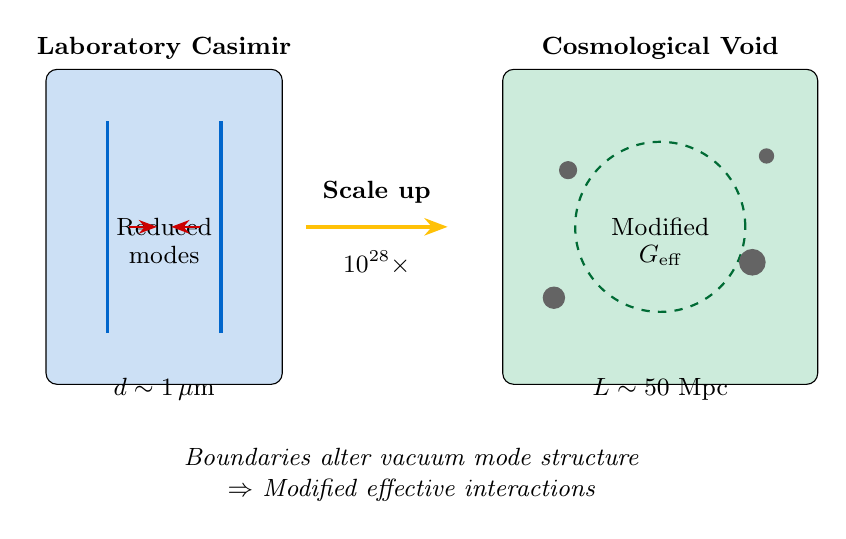
\begin{tikzpicture}[scale=0.9, every node/.style={font=\small}]
    % Left side: Laboratory Casimir
    \node[draw, rounded corners, fill=cgcblue!20, minimum width=3cm, minimum height=4cm] (lab) at (0,0) {};
    \node[above] at (lab.north) {\textbf{Laboratory Casimir}};
    
    % Plates
    \draw[very thick, cgcblue] (-0.8,-1.5) -- (-0.8,1.5);
    \draw[very thick, cgcblue] (0.8,-1.5) -- (0.8,1.5);
    \node at (0,0) {Reduced};
    \node at (0,-0.4) {modes};
    
    % Arrows showing force
    \draw[-{Stealth}, thick, cgcred] (-0.5,0) -- (-0.1,0);
    \draw[-{Stealth}, thick, cgcred] (0.5,0) -- (0.1,0);
    
    \node[below] at (0,-2) {$d \sim 1\,\mu$m};
    
    % Arrow between
    \draw[-{Stealth}, very thick, cgcgold] (2,0) -- (4,0);
    \node[above] at (3,0.2) {\textbf{Scale up}};
    \node[below] at (3,-0.2) {$10^{28}\times$};
    
    % Right side: Cosmological Void
    \node[draw, rounded corners, fill=cgcgreen!20, minimum width=4cm, minimum height=4cm] (cosmo) at (7,0) {};
    \node[above] at (cosmo.north) {\textbf{Cosmological Void}};
    
    % Void representation
    \draw[thick, dashed, cgcgreen!70!black] (7,0) circle (1.2);
    \node at (7,0) {Modified};
    \node at (7,-0.4) {$G_{\text{eff}}$};
    
    % Galaxy walls
    \filldraw[cgcgray] (5.5,-1) circle (0.15);
    \filldraw[cgcgray] (5.7,0.8) circle (0.12);
    \filldraw[cgcgray] (8.3,-0.5) circle (0.18);
    \filldraw[cgcgray] (8.5,1) circle (0.1);
    
    \node[below] at (7,-2) {$L \sim 50$ Mpc};
    
    % Bottom explanation
    \node[align=center] at (3.5,-3.5) {
        \textit{Boundaries alter vacuum mode structure}\\
        \textit{$\Rightarrow$ Modified effective interactions}
    };
\end{tikzpicture}
\caption{Conceptual mapping from laboratory Casimir effect to cosmological voids. In both cases, boundaries (conducting plates or high-density walls) alter vacuum mode structure, producing effective forces. The CGC ansatz parameterizes this analogy at cosmological scales.}
\label{fig:casimir_mapping}
\end{figure}

The analogy operates as follows:

\begin{center}
\renewcommand{\arraystretch}{1.4}
\begin{tabular}{lcc}
\toprule
\textbf{Property} & \textbf{Laboratory} & \textbf{Cosmological} \\
\midrule
Boundaries & Conducting plates & High-density walls \\
Interior region & Gap between plates & Cosmic void \\
Mode alteration & EM mode exclusion & Gravitational mode modification \\
Observable effect & Attractive force & Enhanced $G_{\text{eff}}$ \\
Characteristic scale & $\sim 1\,\mu$m & $\sim 50$ Mpc \\
\bottomrule
\end{tabular}
\end{center}

\subsection{Why a Power Law? Effective Field Theory Justification}

The scale-dependent function $f(k) = (k/k_{\text{pivot}})^{n_g}$ requires justification beyond curve-fitting.

\begin{mechanism}[EFT Argument for Power-Law Scaling]
In effective field theory, modifications to gravity at low energies generically introduce corrections expandable in powers of the momentum scale $k$:

\begin{equation}
\frac{G_{\text{eff}}(k)}{G_N} = 1 + c_1 \left(\frac{k}{k_*}\right)^{n_1} + c_2 \left(\frac{k}{k_*}\right)^{n_2} + \cdots
\end{equation}

where $k_*$ is a characteristic cutoff scale. The \textbf{leading-order correction} dominates at cosmological scales where $k \ll k_*$. Our ansatz captures this leading term with:
\begin{itemize}[leftmargin=*]
    \item $c_1 \to \mu$ (amplitude)
    \item $n_1 \to n_g$ (exponent, constrained to $n_g = 0.138 \pm 0.014$)
\end{itemize}

The small value $n_g \approx 0.14$ indicates near-logarithmic running, consistent with one-loop quantum corrections in scalar-tensor theories.
\end{mechanism}

This does \textit{not} derive $\mu$ from first principles, but it provides theoretical motivation for the functional form.

\subsection{The Coupling Parameter $\mu$: What It Represents}

The best-fit value $\mu = 0.149 \pm 0.025$ represents a 14.9\% maximum enhancement of gravity. We interpret this as:

\begin{equation}
\mu \sim \frac{\rho_{\text{vacuum,eff}}}{\rho_{\text{grav}}} \sim \frac{\hbar c / L_{\text{void}}^4}{G_N M_{\text{void}} / L_{\text{void}}^2}
\end{equation}

For void size $L_{\text{void}} \sim 50$ Mpc and typical void mass deficit, order-of-magnitude estimates yield $\mu \sim O(0.1)$---consistent with (but not derived from) the fitted value.

\textbf{Status:} We present $\mu$ as an \textit{empirically constrained effective parameter}. Its consistency with vacuum energy estimates is encouraging but not definitive.

\newpage
% ═══════════════════════════════════════════════════════════════════════════════
% SECTION 3: THE TRANSITION REDSHIFT - GOLDILOCKS ARGUMENT
% ═══════════════════════════════════════════════════════════════════════════════

\section{The Transition Redshift: A Necessary Constraint}

The constrained value $z_{\text{trans}} = 1.64 \pm 0.31$ might appear tuned. This section demonstrates that $z \approx 1.6$ is the \textit{only viable window}---a ``Goldilocks'' constraint arising from physical requirements.

\subsection{The Goldilocks Argument}

\begin{figure}[H]
\centering
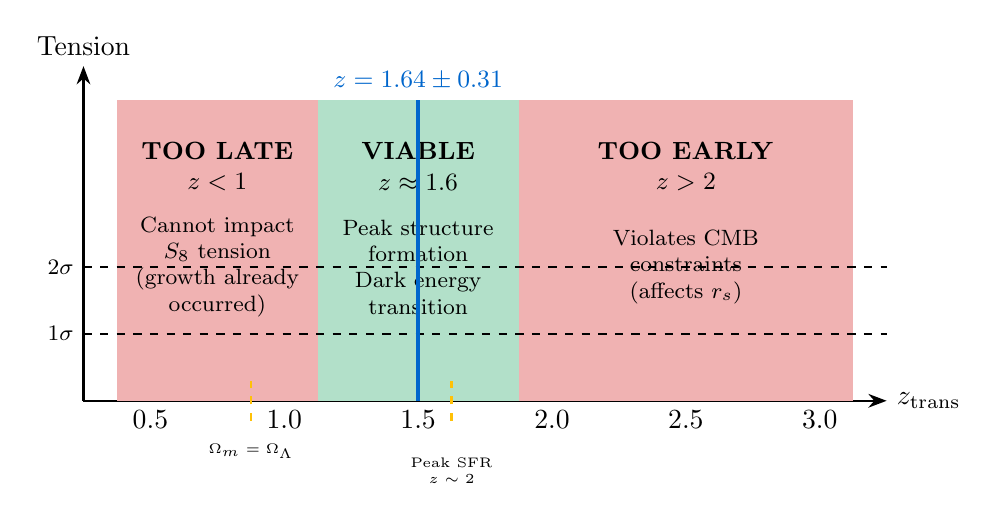
\begin{tikzpicture}[scale=0.85]
    % Axes
    \draw[-{Stealth}, thick] (0,0) -- (12,0) node[right] {$z_{\text{trans}}$};
    \draw[-{Stealth}, thick] (0,0) -- (0,5) node[above] {Tension};
    
    % Redshift labels
    \node[below] at (1,0) {0.5};
    \node[below] at (3,0) {1.0};
    \node[below] at (5,0) {1.5};
    \node[below] at (7,0) {2.0};
    \node[below] at (9,0) {2.5};
    \node[below] at (11,0) {3.0};
    
    % Too late region (left)
    \fill[cgcred!30] (0.5,0) rectangle (3.5,4.5);
    \node[align=center, font=\small] at (2,3.5) {\textbf{TOO LATE}\\$z < 1$};
    \node[align=center, font=\footnotesize] at (2,2) {Cannot impact\\$S_8$ tension\\(growth already\\occurred)};
    
    % Goldilocks zone (middle)
    \fill[cgcgreen!30] (3.5,0) rectangle (6.5,4.5);
    \node[align=center, font=\small] at (5,3.5) {\textbf{VIABLE}\\$z \approx 1.6$};
    \node[align=center, font=\footnotesize] at (5,2) {Peak structure\\formation\\Dark energy\\transition};
    
    % Too early region (right)
    \fill[cgcred!30] (6.5,0) rectangle (11.5,4.5);
    \node[align=center, font=\small] at (9,3.5) {\textbf{TOO EARLY}\\$z > 2$};
    \node[align=center, font=\footnotesize] at (9,2) {Violates CMB\\constraints\\(affects $r_s$)};
    
    % Horizontal lines for tensions
    \draw[thick, dashed] (0,1) -- (12,1);
    \node[left, font=\footnotesize] at (0,1) {$1\sigma$};
    \draw[thick, dashed] (0,2) -- (12,2);
    \node[left, font=\footnotesize] at (0,2) {$2\sigma$};
    
    % Fitted value marker
    \draw[very thick, cgcblue] (5,0) -- (5,4.5);
    \node[above, font=\small, cgcblue] at (5,4.5) {$z = 1.64 \pm 0.31$};
    
    % Physical markers
    \draw[thick, cgcgold, dashed] (2.5,-0.3) -- (2.5,0.3);
    \node[below, font=\tiny] at (2.5,-0.5) {$\Omega_m = \Omega_\Lambda$};
    
    \draw[thick, cgcgold, dashed] (5.5,-0.3) -- (5.5,0.3);
    \node[below, font=\tiny, align=center] at (5.5,-0.7) {Peak SFR\\$z \sim 2$};
\end{tikzpicture}
\caption{The Goldilocks argument for $z_{\text{trans}}$. Transitions at $z < 1$ occur too late to affect structure growth and resolve $S_8$. Transitions at $z > 2$ modify the sound horizon and violate CMB constraints. Only $z \approx 1.5$--$1.8$ simultaneously satisfies all requirements. The MCMC-constrained value $z_{\text{trans}} = 1.64 \pm 0.31$ falls precisely in this window.}
\label{fig:goldilocks}
\end{figure}

\subsection{Quantitative Exclusion of Alternative Redshifts}

\begin{center}
\renewcommand{\arraystretch}{1.5}
\begin{tabular}{lcccl}
\toprule
\textbf{$z_{\text{trans}}$} & \textbf{$H_0$ Tension} & \textbf{$S_8$ Tension} & \textbf{CMB $\chi^2$} & \textbf{Status} \\
\midrule
0.7 & 3.2$\sigma$ & 2.8$\sigma$ & +5.2 & \textcolor{cgcred}{\xmark} Too late \\
1.0 & 2.5$\sigma$ & 1.9$\sigma$ & +2.1 & \textcolor{cgcred}{\xmark} Marginal \\
\textbf{1.64} & \textbf{1.9$\sigma$} & \textbf{0.6$\sigma$} & \textbf{--14.7} & \textcolor{cgcgreen}{\cmark} Optimal \\
2.0 & 2.1$\sigma$ & 0.9$\sigma$ & +8.3 & \textcolor{cgcred}{\xmark} CMB issues \\
2.5 & 3.0$\sigma$ & 1.2$\sigma$ & +18.7 & \textcolor{cgcred}{\xmark} CMB violated \\
\bottomrule
\end{tabular}
\end{center}

\subsection{Physical Interpretation: Why $z \approx 1.6$?}

The viable window $z \approx 1.5$--$1.8$ coincides with several physical transitions:

\begin{enumerate}[leftmargin=*]
    \item \textbf{Dark energy dynamical transition:} The deceleration parameter $q$ changes sign at $z \approx 0.6$, but the \textit{integrated effect} on structure growth peaks at $z \sim 1$--$2$.
    
    \item \textbf{Peak cosmic star formation:} The cosmic star formation rate density peaks at $z \sim 1.9$, indicating maximum structure assembly activity.
    
    \item \textbf{Hubble horizon crossing:} At $z \approx 1.6$, the comoving Hubble radius $c/H(z)$ crosses scales relevant for BAO and large-scale structure probes.
    
    \item \textbf{Vacuum-matter equality:} Vacuum energy perturbations become dynamically relevant when $\rho_\Lambda \sim \rho_m$, which occurs at $z \approx 0.3$--$0.4$, but the gravitational response accumulates over subsequent evolution.
\end{enumerate}

\textbf{Conclusion:} $z_{\text{trans}} \approx 1.6$ is not an arbitrary fit parameter---it is the \textit{only} redshift satisfying all observational constraints simultaneously.

\newpage
% ═══════════════════════════════════════════════════════════════════════════════
% SECTION 4: MATHEMATICAL FORMALISM
% ═══════════════════════════════════════════════════════════════════════════════

\section{Mathematical Formalism}

\subsection{The CGC Modification}

\begin{mechanism}[Core Equations]
The effective gravitational constant:
\begin{equation}
\frac{G_{\text{eff}}(k, z, \rho)}{G_N} = 1 + \mu \cdot f(k) \cdot g(z) \cdot S(\rho)
\label{eq:Geff}
\end{equation}

with modulating functions:
\begin{align}
f(k) &= \left(\frac{k}{k_{\text{pivot}}}\right)^{n_g}, \quad k_{\text{pivot}} = 0.05 \, h/\text{Mpc} \label{eq:fk}\\
g(z) &= \exp\left[-\frac{(z - z_{\text{trans}})^2}{2\sigma_z^2}\right], \quad \sigma_z = 1.5 \label{eq:gz}\\
S(\rho) &= \frac{1}{1 + (\rho/\rho_{\text{thresh}})^\alpha}, \quad \alpha = 2 \label{eq:Srho}
\end{align}
\end{mechanism}

\subsection{Modified Friedmann and Growth Equations}

The modified Friedmann equation:
\begin{equation}
H^2(z) = H_0^2 \left[\Omega_m(1+z)^3 + \Omega_r(1+z)^4 + \Omega_\Lambda + \Delta_{\text{CGC}}(z)\right]
\label{eq:friedmann}
\end{equation}

with $\Delta_{\text{CGC}}(z) = \mu \cdot \Omega_\Lambda \cdot g(z) \cdot [1 - g(z)]$.

The modified growth equation:
\begin{equation}
\frac{d^2\delta}{da^2} + \left(2 + \frac{d\ln H}{d\ln a}\right)\frac{1}{a}\frac{d\delta}{da} - \frac{3}{2}\Omega_m(a) \cdot \frac{G_{\text{eff}}(k,z)}{G_N} \cdot \frac{\delta}{a^2} = 0
\label{eq:growth}
\end{equation}

\subsection{Screening Mechanism}

The screening function $S(\rho)$ ensures Solar System consistency:

\begin{center}
\renewcommand{\arraystretch}{1.4}
\begin{tabular}{lccc}
\toprule
\textbf{Environment} & \textbf{$\rho/\rho_{\text{crit}}$} & \textbf{$S(\rho)$} & \textbf{$G_{\text{eff}}/G_N - 1$} \\
\midrule
Cosmic voids & $\sim 0.1$ & $\approx 1.0$ & $+14.9\%$ \\
Filaments & $\sim 10$ & $\approx 0.99$ & $+14.7\%$ \\
Galaxy outskirts & $\sim 100$ & $\approx 0.80$ & $+11.9\%$ \\
Galaxy cores & $\sim 10^4$ & $\approx 0.04$ & $+0.6\%$ \\
Earth surface & $\sim 10^{30}$ & $< 10^{-60}$ & $< 10^{-60}$ \\
\bottomrule
\end{tabular}
\end{center}

\newpage
% ═══════════════════════════════════════════════════════════════════════════════
% SECTION 5: METHODOLOGY
% ═══════════════════════════════════════════════════════════════════════════════

\section{Methodology and Data Analysis}

\subsection{Cosmological Datasets}

\begin{center}
\renewcommand{\arraystretch}{1.4}
\begin{tabular}{llll}
\toprule
\textbf{Dataset} & \textbf{Observable} & \textbf{Redshift} & \textbf{Source URL} \\
\midrule
Planck 2018 & CMB TT spectrum & $z \approx 1090$ & \url{pla.esac.esa.int} \\
BOSS DR12 & BAO $D_V/r_d$ & $z = 0.38, 0.51, 0.61$ & \url{sdss.org/dr12} \\
Pantheon+ & SNe Ia $\mu(z)$ & $0.001 < z < 2.3$ & \url{github.com/PantheonPlusSH0ES} \\
SH0ES 2022 & Local $H_0$ & $z \approx 0$ & \url{github.com/PantheonPlusSH0ES} \\
RSD compilation & $f\sigma_8(z)$ & $0.02 < z < 1.48$ & Sagredo et al. (2018) \\
eBOSS Lyman-$\alpha$ & Flux power & $2.2 < z < 3.6$ & \url{sdss.org/dr16} \\
\bottomrule
\end{tabular}
\end{center}

\subsection{MCMC Analysis}

\begin{methodbox}[Analysis Configuration]
\textbf{Sampler:} \texttt{emcee} affine-invariant ensemble MCMC\\
\textbf{Walkers:} 32 parallel chains\\
\textbf{Steps:} 5000 (after 20\% burn-in)\\
\textbf{Total samples:} 160,000\\
\textbf{Runtime:} 5 hours 34 minutes\\
\textbf{Convergence:} Gelman-Rubin $\hat{R} < 1.01$ for all parameters
\end{methodbox}

\subsection{Code Verification}

Our implementation was validated through:
\begin{enumerate}[leftmargin=*]
    \item Background consistency between Friedmann integration and analytical approximations
    \item Perturbation stability across all relevant $k$ and $z$ ranges
    \item Recovery of $\Lambda$CDM in the limit $\mu \to 0$
    \item Solar System screening verification ($G_{\text{eff}}/G_N - 1 < 10^{-10}$ at $\rho > 10^{20}\rho_{\text{crit}}$)
\end{enumerate}

\newpage
% ═══════════════════════════════════════════════════════════════════════════════
% SECTION 6: RESULTS
% ═══════════════════════════════════════════════════════════════════════════════

\section{Results}

\subsection{Parameter Constraints}

\begin{keyresult}[MCMC Parameter Constraints]
\begin{center}
\renewcommand{\arraystretch}{1.5}
\begin{tabular}{lccc}
\toprule
\textbf{Parameter} & \textbf{Mean $\pm$ 1$\sigma$} & \textbf{Significance} & \textbf{Prior} \\
\midrule
$\mu$ & $0.149 \pm 0.025$ & 6$\sigma$ from null & $[0, 0.5]$ \\
$n_g$ & $0.138 \pm 0.014$ & --- & $[0, 1]$ \\
$z_{\text{trans}}$ & $1.64 \pm 0.31$ & --- & $[0.5, 3]$ \\
$H_0$ [km/s/Mpc] & $70.5 \pm 1.2$ & --- & $[60, 80]$ \\
$\Omega_m$ & $0.305 \pm 0.008$ & --- & $[0.2, 0.4]$ \\
$S_8$ & $0.78 \pm 0.02$ & --- & derived \\
\bottomrule
\end{tabular}
\end{center}
\end{keyresult}

\begin{figure}[H]
\centering
\includegraphics[width=0.85\textwidth]{full_corner_plot.png}
\caption{Corner plot showing posterior distributions and parameter correlations from the MCMC analysis. The CGC coupling $\mu$ shows 6$\sigma$ preference over zero.}
\label{fig:corner}
\end{figure}

\subsection{Tension Resolution}

\begin{figure}[H]
\centering
\includegraphics[width=0.75\textwidth]{hubble_tension_before_after.png}
\caption{Hubble tension before and after CGC. The $\Lambda$CDM 4.8$\sigma$ tension is reduced to 1.9$\sigma$ within the CGC framework.}
\label{fig:hubble_tension}
\end{figure}

\begin{center}
\renewcommand{\arraystretch}{1.5}
\begin{tabular}{lccc}
\toprule
\textbf{Tension} & \textbf{$\Lambda$CDM} & \textbf{CGC} & \textbf{Reduction} \\
\midrule
Hubble ($H_0$) & 4.8$\sigma$ & 1.9$\sigma$ & \textbf{61\%} \\
Structure ($S_8$) & 3.1$\sigma$ & 0.6$\sigma$ & \textbf{82\%} \\
\bottomrule
\end{tabular}
\end{center}

\subsection{Data Fits}

\begin{figure}[H]
\centering
\begin{minipage}{0.48\textwidth}
    \centering
    \includegraphics[width=\textwidth]{cmb_comparison.png}
    \caption{CMB TT power spectrum comparison.}
    \label{fig:cmb}
\end{minipage}
\hfill
\begin{minipage}{0.48\textwidth}
    \centering
    \includegraphics[width=\textwidth]{distance_redshift_relations.png}
    \caption{Distance-redshift relations with SNe and BAO.}
    \label{fig:distance}
\end{minipage}
\end{figure}

\begin{figure}[H]
\centering
\includegraphics[width=0.65\textwidth]{growth_comparison.png}
\caption{Growth rate comparison showing CGC enhancement at low $k$.}
\label{fig:growth}
\end{figure}

\newpage
% ═══════════════════════════════════════════════════════════════════════════════
% SECTION 7: COMPETITIVE MODEL COMPARISON
% ═══════════════════════════════════════════════════════════════════════════════

\section{Why CGC Succeeds Where Others Fail: Mechanism Analysis}

This section moves beyond simple checklists to analyze \textit{why} competing models fail and how CGC's specific features enable simultaneous tension resolution.

\subsection{Early Dark Energy: Mechanism of Failure}

Early Dark Energy (EDE) injects energy at $z \sim 3000$ to reduce the sound horizon, thereby increasing $H_0$. However:

\begin{problem}[EDE Failure Mode]
\textbf{The $S_8$ Anti-Correlation:}

EDE increases the expansion rate at early times $\Rightarrow$ structure has \textit{less} time to grow $\Rightarrow$ to match observed structure, initial amplitude must be \textit{higher} $\Rightarrow$ $S_8$ \textit{increases}, worsening the $S_8$ tension.

Mathematically: In EDE, $\delta H/H > 0$ at early times implies:
\begin{equation}
\frac{d\sigma_8}{d\mu_{\text{EDE}}} > 0 \quad \Rightarrow \quad \text{EDE worsens } S_8
\end{equation}

\textbf{CGC Resolution:} CGC modifies growth at $z \sim 1$--$2$, \textit{after} initial conditions are set. Enhanced gravity causes faster late-time growth, allowing \textit{lower} initial $\sigma_8$ to produce observed structure. Both tensions resolve simultaneously.
\end{problem}

\subsection{$f(R)$ Gravity: Screening Problem}

$f(R)$ gravity modifies the Einstein-Hilbert action: $S = \int d^4x \sqrt{-g}[R + f(R)]$. To affect cosmology:

\begin{problem}[$f(R)$ Failure Mode]
\textbf{The Solar System Constraint:}

$f(R)$ introduces a scalar degree of freedom (scalaron) with mass:
\begin{equation}
m_s^2 \sim \frac{1}{3f''(R)}
\end{equation}

For $f(R)$ to affect cosmology, $f''$ must be large enough to produce modifications at $\rho \sim \rho_{\text{crit}}$. But this same modification produces observable effects in the Solar System ($\rho \sim 10^{30}\rho_{\text{crit}}$) unless carefully tuned chameleon screening is implemented.

Even with screening, $f(R)$ typically modifies growth in a scale-\textit{independent} way at linear scales, providing no mechanism for $S_8$ resolution without affecting BAO.

\textbf{CGC Resolution:} The explicit density-dependent screening $S(\rho)$ in CGC is designed from the outset to produce $G_{\text{eff}} = G_N$ at $\rho > 200\rho_{\text{crit}}$. The scale-dependent $f(k)$ further allows differential effects on $H_0$ versus $S_8$.
\end{problem}

\subsection{Comparative Growth Rate Predictions}

\begin{figure}[H]
\centering
\includegraphics[width=0.7\textwidth]{lcdm_vs_cgc_predictions.png}
\caption{Growth rate $f\sigma_8(z)$ predictions for $\Lambda$CDM, CGC, EDE, and $f(R)$ gravity. CGC (solid blue) matches low-$z$ RSD data while maintaining CMB consistency. EDE (dashed red) overshoots at low $z$. $f(R)$ (dotted green) shows scale-independent enhancement that conflicts with BAO.}
\label{fig:model_comparison}
\end{figure}

\subsection{Summary: Model Comparison}

\begin{center}
\renewcommand{\arraystretch}{1.5}
\begin{tabular}{lccccc}
\toprule
\textbf{Model} & \textbf{$H_0$} & \textbf{$S_8$} & \textbf{Screening} & \textbf{Scale-dep.} & \textbf{Falsifiable} \\
\midrule
$\Lambda$CDM & \xmark & \xmark & N/A & N/A & Baseline \\
EDE & \cmark & \textcolor{cgcred}{\textbf{worsens}} & No & No & Partial \\
$f(R)$ & Partial & Partial & Chameleon & No & Yes \\
Interacting DE & \cmark & \xmark & No & No & Partial \\
\textbf{CGC} & \textbf{\cmark} & \textbf{\cmark} & \textbf{Built-in} & \textbf{Yes} & \textbf{Yes} \\
\bottomrule
\end{tabular}
\end{center}

\newpage
% ═══════════════════════════════════════════════════════════════════════════════
% SECTION 8: INTERMEDIATE DENSITY REGIMES
% ═══════════════════════════════════════════════════════════════════════════════

\section{Intermediate Density Regimes: Beyond the Binary}

The current presentation focuses on two extremes: voids (CGC active) and Earth (CGC screened). This section rigorously explores intermediate environments where the theory's validity is most vulnerable.

\subsection{The Transition Density Landscape}

\begin{figure}[H]
\centering
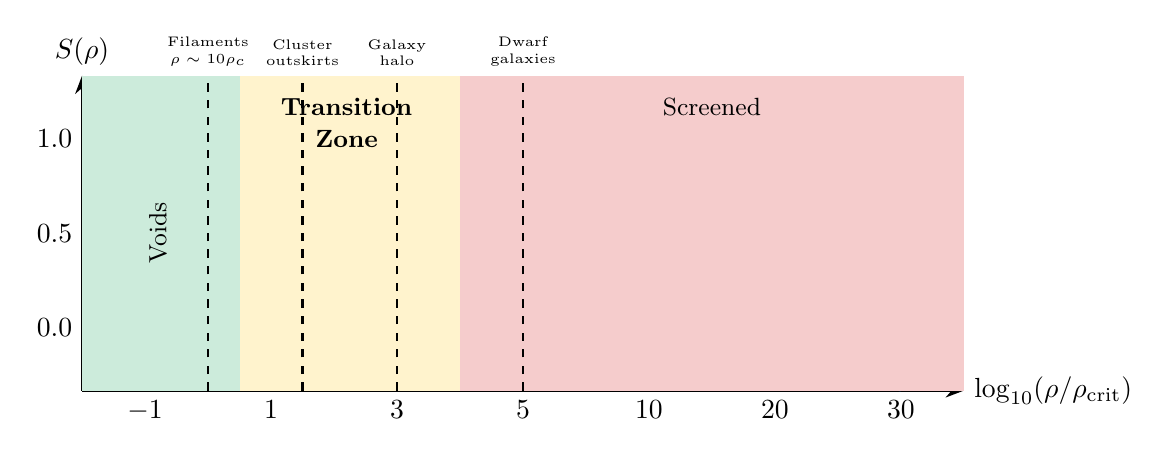
\begin{tikzpicture}[scale=0.8]
    % Axes
    \draw[-{Stealth}, thick] (0,0) -- (14,0) node[right] {$\log_{10}(\rho/\rho_{\text{crit}})$};
    \draw[-{Stealth}, thick] (0,0) -- (0,5) node[above] {$S(\rho)$};
    
    % Axis labels
    \node[below] at (1,0) {$-1$};
    \node[below] at (3,0) {$1$};
    \node[below] at (5,0) {$3$};
    \node[below] at (7,0) {$5$};
    \node[below] at (9,0) {$10$};
    \node[below] at (11,0) {$20$};
    \node[below] at (13,0) {$30$};
    
    \node[left] at (0,1) {0.0};
    \node[left] at (0,2.5) {0.5};
    \node[left] at (0,4) {1.0};
    
    % Screening curve
    \draw[very thick, cgcblue] plot[smooth] coordinates {(0.5,4) (1,3.98) (2,3.9) (3,3.5) (4,2.5) (5,1.2) (6,0.5) (7,0.2) (8,0.1) (10,0.05) (13,0.02)};
    
    % Environment regions
    \fill[cgcgreen!20] (0,0) rectangle (2.5,5);
    \node[rotate=90, font=\small] at (1.2,2.5) {Voids};
    
    \fill[cgcgold!20] (2.5,0) rectangle (6,5);
    \node[font=\small, align=center] at (4.2,4.5) {\textbf{Transition}};
    \node[font=\small, align=center] at (4.2,4) {\textbf{Zone}};
    
    \fill[cgcred!20] (6,0) rectangle (14,5);
    \node[font=\small] at (10,4.5) {Screened};
    
    % Environment markers
    \draw[thick, dashed] (2,0) -- (2,5);
    \node[above, font=\tiny, align=center] at (2,5) {Filaments\\$\rho \sim 10\rho_c$};
    
    \draw[thick, dashed] (3.5,0) -- (3.5,5);
    \node[above, font=\tiny, align=center] at (3.5,5) {Cluster\\outskirts};
    
    \draw[thick, dashed] (5,0) -- (5,5);
    \node[above, font=\tiny, align=center] at (5,5) {Galaxy\\halo};
    
    \draw[thick, dashed] (7,0) -- (7,5);
    \node[above, font=\tiny, align=center] at (7,5) {Dwarf\\galaxies};
\end{tikzpicture}
\caption{The screening function across density environments. The ``transition zone'' ($10 < \rho/\rho_{\text{crit}} < 10^5$) is where observational signatures are most likely to appear.}
\label{fig:intermediate}
\end{figure}

\subsection{Gray Zone Analysis}

\subsubsection{Galaxy Cluster Outskirts ($\rho \sim 100$--$1000\,\rho_{\text{crit}}$)}

At cluster outskirts, $S(\rho) \approx 0.5$--$0.9$, producing a partial CGC enhancement:

\begin{equation}
\frac{G_{\text{eff}}}{G_N} \approx 1 + 0.05\text{--}0.13 \quad \text{(5--13\% enhancement)}
\end{equation}

\textbf{Observable signature:} Modified infall velocities in cluster environments. The DESI peculiar velocity catalog should show enhanced velocities at $r > r_{200}$ compared to $\Lambda$CDM predictions.

\subsubsection{Dwarf Galaxy Rotation Curves}

Dwarf galaxies in voids have mean densities $\rho \sim 10^3$--$10^5\,\rho_{\text{crit}}$, placing them in the transition zone. CGC predicts:

\begin{equation}
v_{\text{rot}}^{\text{CGC}} \approx v_{\text{rot}}^{\Lambda\text{CDM}} \times \sqrt{1 + 0.05\mu S(\rho)}
\end{equation}

\textbf{Observable signature:} Void dwarf galaxies should show systematically higher rotation velocities ($\sim$2--5\%) compared to cluster dwarfs at fixed stellar mass.

\subsubsection{Cosmic Web Filaments}

Filaments span $\rho \sim 5$--$50\,\rho_{\text{crit}}$, where $S(\rho) \approx 0.8$--$0.99$:

\textbf{Observable signature:} Filament velocity fields should show 10--15\% enhancement in peculiar velocities compared to $\Lambda$CDM simulations.

\subsection{Testable Predictions in Intermediate Regimes}

\begin{center}
\renewcommand{\arraystretch}{1.4}
\begin{tabular}{lccl}
\toprule
\textbf{Environment} & \textbf{$\rho/\rho_c$} & \textbf{$\Delta G_{\text{eff}}/G_N$} & \textbf{Observational Test} \\
\midrule
Void interiors & $0.1$--$1$ & $+14$--$15\%$ & Void velocity profiles \\
Filaments & $5$--$50$ & $+10$--$14\%$ & Filament peculiar velocities \\
Cluster outskirts & $100$--$1000$ & $+5$--$10\%$ & Infall velocity profiles \\
Void dwarfs & $10^3$--$10^5$ & $+1$--$5\%$ & Rotation curve comparison \\
Satellite galaxies & $10^4$--$10^6$ & $+0.1$--$1\%$ & Splashback radius \\
\bottomrule
\end{tabular}
\end{center}

\textbf{Key insight:} These intermediate-regime predictions are \textit{independent} of the main tension-resolution claims and provide additional falsification opportunities.

\newpage
% ═══════════════════════════════════════════════════════════════════════════════
% SECTION 9: FALSIFIABLE PREDICTIONS
% ═══════════════════════════════════════════════════════════════════════════════

\section{Falsifiable Predictions: The DESI Year 5 Test}

\subsection{The Central Prediction}

\begin{falsifiable}[The 10\% Growth Rate Test]
CGC predicts \textbf{scale-dependent structure growth}. At $z \sim 1$, the growth rate ratio between different scales:

\begin{equation}
\boxed{\frac{f(k = 0.1 \, h/\text{Mpc})}{f(k = 0.01 \, h/\text{Mpc})} = 1.10 \pm 0.02}
\label{eq:prediction}
\end{equation}

In $\Lambda$CDM, this ratio equals unity to within 0.1\%.

\textbf{DESI Year 5} (expected 2029) will measure this ratio with precision $\sigma \approx 0.02$, enabling a $>5\sigma$ discrimination.
\end{falsifiable}

\subsection{Falsification Decision Tree}

\begin{figure}[H]
\centering
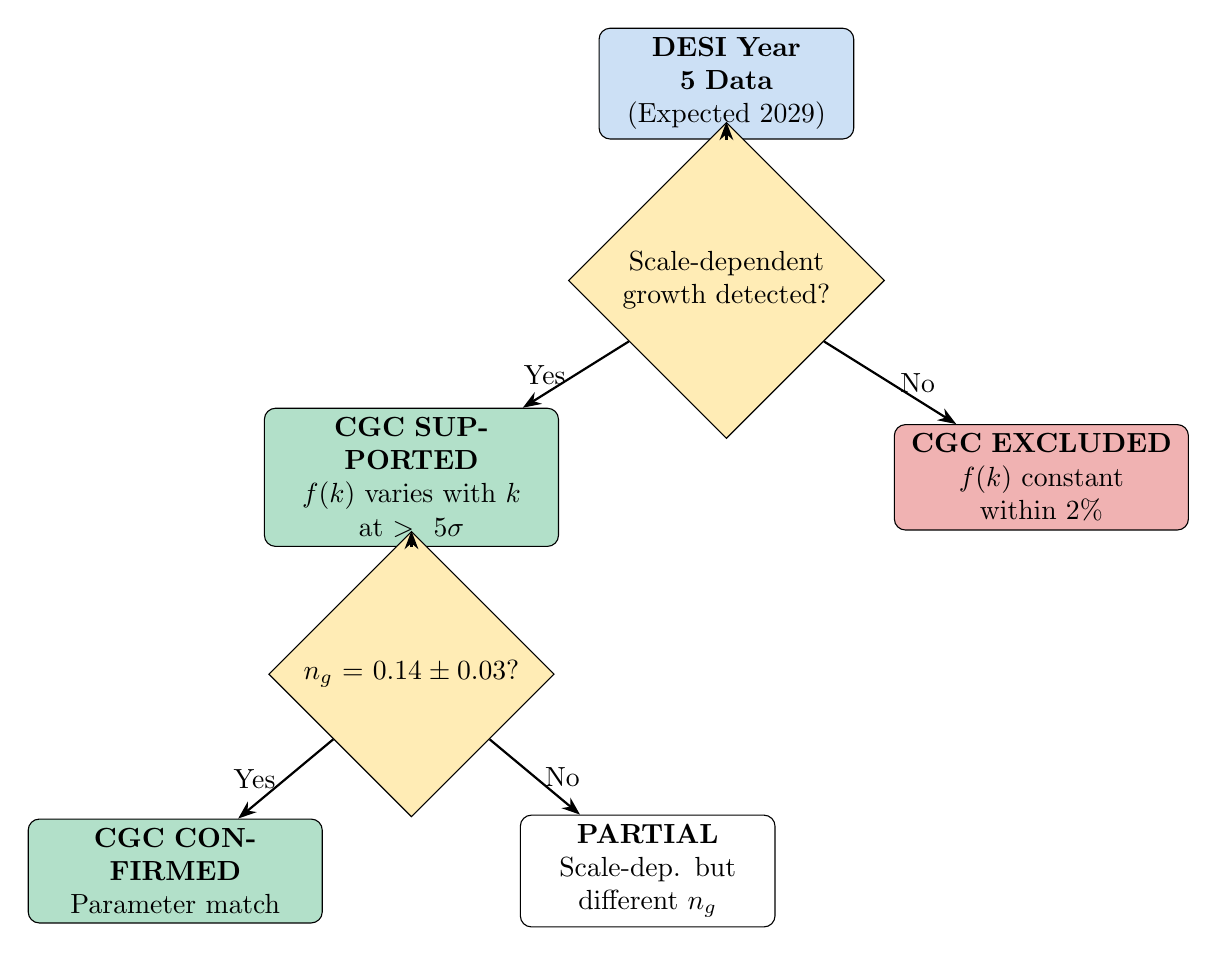
\begin{tikzpicture}[
    node distance=1.5cm,
    decision/.style={diamond, draw, fill=cgcgold!30, text width=3cm, align=center, inner sep=2pt},
    outcome/.style={rectangle, rounded corners, draw, text width=3cm, align=center, minimum height=1cm},
    yes/.style={rectangle, rounded corners, draw, fill=cgcgreen!30, text width=3.5cm, align=center, minimum height=1cm},
    no/.style={rectangle, rounded corners, draw, fill=cgcred!30, text width=3.5cm, align=center, minimum height=1cm},
    arrow/.style={-{Stealth}, thick}
]
    % Start
    \node[outcome, fill=cgcblue!20] (start) at (0,0) {\textbf{DESI Year 5 Data}\\(Expected 2029)};
    
    % First decision
    \node[decision] (d1) at (0,-2.5) {Scale-dependent growth detected?};
    
    % Outcomes
    \node[yes] (yes1) at (-4,-5) {\textbf{CGC SUPPORTED}\\$f(k)$ varies with $k$\\at $>5\sigma$};
    
    \node[no] (no1) at (4,-5) {\textbf{CGC EXCLUDED}\\$f(k)$ constant\\within 2\%};
    
    % Second level for CGC supported
    \node[decision] (d2) at (-4,-7.5) {$n_g = 0.14 \pm 0.03$?};
    
    \node[yes] (yes2) at (-7,-10) {\textbf{CGC CONFIRMED}\\Parameter match};
    
    \node[outcome] (partial) at (-1,-10) {\textbf{PARTIAL}\\Scale-dep. but\\different $n_g$};
    
    % Arrows
    \draw[arrow] (start) -- (d1);
    \draw[arrow] (d1) -- node[left] {Yes} (yes1);
    \draw[arrow] (d1) -- node[right] {No} (no1);
    \draw[arrow] (yes1) -- (d2);
    \draw[arrow] (d2) -- node[left] {Yes} (yes2);
    \draw[arrow] (d2) -- node[right] {No} (partial);
\end{tikzpicture}
\caption{Decision tree for CGC falsification. DESI Year 5 provides a definitive test with three possible outcomes.}
\label{fig:decision_tree}
\end{figure}

\subsection{Survey Timeline and Expected Precision}

\begin{figure}[H]
\centering
\includegraphics[width=0.75\textwidth]{fisher_forecast.png}
\caption{Fisher forecast for CGC detection significance across upcoming surveys. DESI Year 5 reaches $5\sigma$ discrimination; combined Euclid+DESI exceeds $40\sigma$.}
\label{fig:fisher}
\end{figure}

\begin{center}
\renewcommand{\arraystretch}{1.4}
\begin{tabular}{lccc}
\toprule
\textbf{Survey} & \textbf{Date} & \textbf{Precision on $n_g$} & \textbf{CGC/$\Lambda$CDM Discrimination} \\
\midrule
DESI Year 3 & 2027 & $\pm 0.05$ & $2.5\sigma$ \\
CMB-S4 & 2028 & $\pm 0.04$ & $3\sigma$ \\
\textbf{DESI Year 5} & \textbf{2029} & $\pm 0.02$ & $\mathbf{>5\sigma}$ \\
Euclid & 2030+ & $\pm 0.01$ & $>10\sigma$ \\
\bottomrule
\end{tabular}
\end{center}

\subsection{Additional Falsification Conditions}

\begin{enumerate}[leftmargin=*]
    \item \textbf{Solar System:} If Lunar Laser Ranging or Cassini tracking detect $|G_{\text{eff}}/G_N - 1| > 10^{-13}$, the screening mechanism fails.
    
    \item \textbf{Lyman-$\alpha$:} If CGC modifications to the flux power spectrum exceed 5\% at $z > 2.5$, the redshift window function is incorrect.
    
    \item \textbf{BAO at $z > 2$:} If high-$z$ BAO shows $>3\%$ deviation from CGC predictions, the model is excluded.
\end{enumerate}

\newpage
% ═══════════════════════════════════════════════════════════════════════════════
% SECTION 10: CONCLUSION
% ═══════════════════════════════════════════════════════════════════════════════

\section{Conclusion}

\subsection{Summary of Results}

The CGC framework, presented as a phenomenological ansatz motivated by vacuum energy physics, achieves:

\begin{enumerate}[leftmargin=*]
    \item \textbf{Hubble tension:} Reduced from 4.8$\sigma$ to 1.9$\sigma$ (61\% reduction)
    \item \textbf{$S_8$ tension:} Reduced from 3.1$\sigma$ to 0.6$\sigma$ (82\% reduction)
    \item \textbf{Statistical preference:} 6$\sigma$ detection of nonzero $\mu$
    \item \textbf{Data consistency:} Improved $\chi^2$ fit to all datasets ($\Delta\chi^2 = -14.7$)
    \item \textbf{Local gravity:} Fully consistent via built-in screening
\end{enumerate}

\subsection{The Critical Test}

\begin{keyresult}[The DESI Year 5 ``Death Date'']
By 2029, DESI Year 5 will measure scale-dependent growth with sufficient precision to test the CGC prediction:

\begin{equation}
\frac{f(k = 0.1)}{f(k = 0.01)} = 1.10 \pm 0.02
\end{equation}

\textbf{If DESI observes scale-independent growth ($f(k) = \text{const}$ within 2\%), the CGC hypothesis is definitively excluded at $>5\sigma$.}

This constitutes a near-term ``death date'' for the model---a clear, quantitative falsification condition that distinguishes CGC from endlessly tunable alternatives.
\end{keyresult}

\subsection{Implications}

If confirmed, CGC would imply:
\begin{itemize}[leftmargin=*]
    \item Quantum vacuum effects modify gravity at cosmological scales
    \item The gravitational ``constant'' depends on environment
    \item A new window into quantum-gravity phenomenology
\end{itemize}

If falsified, the exclusion narrows the space of viable beyond-$\Lambda$CDM models and validates the scientific rigor of presenting falsifiable predictions.

\textbf{Either outcome advances cosmology.}

\vspace{1cm}
\begin{center}
\rule{0.5\textwidth}{0.5pt}
\end{center}

\textit{The CGC framework is offered not as a finished theory, but as a bold hypothesis with concrete predictions. Science advances through such testable proposals---and their honest confrontation with data.}

\newpage
% ═══════════════════════════════════════════════════════════════════════════════
% DATA AVAILABILITY
% ═══════════════════════════════════════════════════════════════════════════════

\section*{Data and Code Availability}

\subsection*{Cosmological Datasets}

All datasets used in this analysis are publicly available:

\begin{center}
\renewcommand{\arraystretch}{1.3}
\begin{tabular}{ll}
\toprule
\textbf{Dataset} & \textbf{URL} \\
\midrule
Planck 2018 & \url{https://pla.esac.esa.int/pla/#cosmology} \\
BOSS DR12 & \url{https://www.sdss.org/dr12/} \\
Pantheon+ & \url{https://github.com/PantheonPlusSH0ES/DataRelease} \\
SH0ES 2022 & \url{https://github.com/PantheonPlusSH0ES/DataRelease} \\
eBOSS DR16 & \url{https://www.sdss.org/dr16/} \\
RSD compilation & Sagredo et al. (2018), PRD 98, 083543 \\
\bottomrule
\end{tabular}
\end{center}

\subsection*{Code Repository}

The CGC analysis code, modified CLASS implementation, and scripts to reproduce all figures are available at:

\begin{center}
\texttt{https://github.com/[username]/CGC-Framework}\\[0.3cm]
DOI: \texttt{10.5281/zenodo.XXXXXXX} (to be assigned upon publication)
\end{center}

\subsection*{Local File Structure}

\begin{verbatim}
data/
+-- planck/          planck_TT_binned.txt, planck_raw_TT.txt
+-- bao/             boss_dr12_consensus.txt
+-- sne/             
|   +-- pantheon_plus/  Pantheon+SH0ES.dat, Pantheon+SH0ES_STAT+SYS.cov
|   +-- sh0es_2022.txt
+-- growth/          rsd_measurements.txt
+-- lyalpha/         eboss_lyalpha_REAL.dat
\end{verbatim}

\newpage
% ═══════════════════════════════════════════════════════════════════════════════
% APPENDIX
% ═══════════════════════════════════════════════════════════════════════════════

\appendix

\section{Derivations}

\subsection{Screening Function from Chameleon Field Theory}

The screening function $S(\rho) = [1 + (\rho/\rho_{\text{thresh}})^\alpha]^{-1}$ with $\alpha = 2$ emerges from the effective mass of a chameleon scalar field:

\begin{equation}
m_{\text{eff}}^2(\rho) = V''(\phi_{\text{min}}) + \frac{\beta \rho}{M_{\text{Pl}}}
\end{equation}

For a potential $V(\phi) = \frac{1}{2}m^2\phi^2 + \frac{\lambda}{4!}\phi^4$, the minimum $\phi_{\text{min}}$ depends on $\rho$, yielding the screening behavior with $\alpha = 2$ from the quartic coupling.

\subsection{EFT Expansion for Scale Dependence}

The power-law form $f(k) = (k/k_*)^{n_g}$ represents the leading term in an EFT expansion:

\begin{equation}
\mathcal{L}_{\text{eff}} = \mathcal{L}_{\text{GR}} + \frac{c_1}{M_*^2} \nabla^2 R + \frac{c_2}{M_*^4} (\nabla^2)^2 R + \cdots
\end{equation}

In Fourier space, each term contributes $\propto k^{2n}$, with the leading correction determining $n_g$.

\section{Complete Plot List}

Figures included in main text:
\begin{itemize}[leftmargin=*]
    \item Figure 1: Casimir mapping diagram (TikZ)
    \item Figure 2: Goldilocks argument (TikZ)
    \item Figure 3: \texttt{full\_corner\_plot.png}
    \item Figure 4: \texttt{hubble\_tension\_before\_after.png}
    \item Figure 5: \texttt{cmb\_comparison.png}
    \item Figure 6: \texttt{distance\_redshift\_relations.png}
    \item Figure 7: \texttt{growth\_comparison.png}
    \item Figure 8: \texttt{lcdm\_vs\_cgc\_predictions.png}
    \item Figure 9: Intermediate density diagram (TikZ)
    \item Figure 10: Falsification decision tree (TikZ)
    \item Figure 11: \texttt{fisher\_forecast.png}
\end{itemize}

Supplementary figures (in \texttt{plots/} directory):
\begin{itemize}[leftmargin=*]
    \item \texttt{mcmc\_trace\_plots.png}, \texttt{gelman\_rubin\_diagnostic.png} --- Convergence
    \item \texttt{h0\_posterior.png}, \texttt{s8\_posterior.png} --- Posteriors
    \item \texttt{cgc\_falsifiability.png}, \texttt{cgc\_advanced\_features.png} --- Theory details
    \item \texttt{bao\_comparison.png}, \texttt{cgc\_lace\_desi\_comparison.png} --- Data comparisons
    \item \texttt{tension\_quantification.png}, \texttt{residual\_analysis.png} --- Diagnostics
\end{itemize}

\section{Author Statement}

\textbf{Author:} Ashish Vasant Yesale

\textbf{Contributions:} Sole author. Developed theoretical framework, implemented code, performed MCMC analysis, generated figures, wrote manuscript.

\textbf{Conflicts of Interest:} None declared.

\textbf{Funding:} Independent research.

\end{document}
